\documentclass[Afour,sageh,times]{sagej}

\usepackage{moreverb,url}

\usepackage[colorlinks,bookmarksopen,bookmarksnumbered,citecolor=red,urlcolor=red]{hyperref}

\newcommand\BibTeX{{\rmfamily B\kern-.05em \textsc{i\kern-.025em b}\kern-.08em
T\kern-.1667em\lower.7ex\hbox{E}\kern-.125emX}}

\def\volumeyear{2023}

\begin{document}

\runninghead{Shabayek, Théro, Almanla, Vincent}

%\title{Misinformation policies of large platforms: methods \& illustration}
\title{Misinformation policies of large platforms: methods and illustration}

\author{Shaden Shabayek\affilnum{1}, H\'{e}lo\"{i}se Th\'{e}ro\affilnum{2}, Dana Almanla\affilnum{3}, Emmanuel Vincent\affilnum{4}}

\affiliation{\affilnum{1}Post-doctoral researcher at Universit\'{e} Paris-Saclay \& associate researcher at Medialab SciencesPo\\
\affilnum{2} xxxx \\ 
\affilnum{3} xxxx \\
\affilnum{4} xxxx}

\corrauth{Shaden Shabayek}

\email{shaden.shabayek@sciencespo.fr}

\begin{abstract}
There is growing pressure for very large online platforms, such as Facebook, Twitter or YouTube, to deal with misinformation by moderating content deemed as harmful and misleading. We investigate platforms' interventions by collecting social media data via APIs and scraping. These interventions can be classified into three broad categories: (i) displaying flags and information panels,  (ii) reducing the visibility of content at the post or account level and (iii) temporary or permanent suspension of users and content deletion. We provide examples illustrating how researchers can monitor misinformation related interventions within each of these three categories. Finally, we discuss the restrictions to access data, the lack of meaningful transparency and the necessity of independent audits.
\end{abstract}

\keywords{Misinformation, content moderation, large platforms.}

\maketitle

\section{Introduction}

Section $230$ in the Communications Decency Act (1996) in the US and articles $12$ and $15$ in the e-commerce Directive (2000) in the EU,  provide immunity for website platforms against the content created by users. This regulatory framework was meant to help internet service providers and online intermediaries to develop. About two decades later, the initial project of a decentralised internet where users can communicate, express themselves, acquire and build collectively new knowledge, has been replaced by a centralised cyberspace dominated by a handful of tech giants.  This market concentration has been accompanied over the years by growing concerns about informational disorders, including the propagation of misleading content concerning matters of public interest or the normalisation of hate speech. Being subject to public pressure, large social media platforms, such as Facebook, Twitter or YouTube, have adopted a model of self-regulation to tackle these informational disorders and have each practiced some form of content moderation (see \cite{gillespie2018custodians} and  \cite{kaye2019speech} for a discussion). Namely, large platforms have tailored {\it terms of service} that users are bound to respect in order to be able to use the offered products, such as access to one's account or the possibility to publish content. Large platforms themselves are in charge of making sure these rules are not violated. In particular, they take explicit actions when content is in violation of local laws in different jurisdictions, such as laws regarding defamation of a racial nature or privacy protection.\endnote{Facebook reports having implemented a total of $64.7$ thousand content restrictions based on local law across all countries in 2020. See Facebook Transparency Center, Content restrictions based on Local Law: \href{https://transparency.fb.com/data/content\-restrictions}{transparency.fb.com/data/content\-restrictions}. We summed the count of content restrictions over all countries reported in the table, for $H1$ and $H2$ of the year 2020.} While each large platform has its own original identity as a private company which provides means of communication and a space for expression for millions of users worldwide, their growing influence on public conversations has made several actors question their legitimacy and capacity to govern what has come to be a new online public sphere. The recent adoption of the Digital Services Act (hereafter \cite{dsa}) in Europe marks a shift in paradigm, as the transparency and accountability of large platforms constitute the main pillars of this new regulatory framework, see \cite{hoboken2022dsa} for a discussion about enforcement. 
% focus: too big to let them be on their own 
% toO big, big impact , that their could be big harm that collective effort is needed to govern this space.
% work has been done on policy areas nudity child safety etc mdoerators + algorithms but not misleading content a big issue that we cant rly handle ? 

\smallskip

Community guidelines of Facebook, Twitter and YouTube can be summarised in a handful of categories, regarding safety, privacy and authenticity; which include sub-categories such as violence, terrorism, child sexual exploitation, abuse, harassment, hateful conduct, suicide or self-harm, illegal or regulated goods and services, platform manipulation and spam. While specific to each platform, the previously cited categories correspond in most cases to well defined concepts, for which there exists legal frameworks in many countries. However, misleading content suffers from a lack of a pertinent and consensual definition (\cite{fathaigh}, \cite{lazer}) and is often subject to misconceptions (\cite{Berriche2023}). It is difficult to identify and qualify a piece of online content as inaccurate, misleading and harmful, among a large volume of daily produced content including opinions, satire and parody. During the COVID-19 global health pandemic, platforms have upgraded their guidelines to include a set of rules to tackle the propagation of potentially harmful content. One novel policy by \cite{facebookcovid} and \cite{twittercovid} consisted in listing a number of claims deemed as misleading or false and announcing clearly that the platform will remove these statements. \endnote{Notice that for Twitter the Policy has been suspended since November 23, 2022.}
%\endnote{See the archived version of Facebook's covid 19 policy \href{https://archive.ph/PaQW8}{https://archive.ph/PaQW8}. Notice that for Twitter the Policy has been suspended since November 23, 2022. See \href{https://archive.ph/ez3eO}{https://archive.ph/ez3eO}.} 
Such targeted policies show the willingness of mainstream platforms to enhance the quality of the online conversation. Yet it also sheds light on the lack of specific consensual policies to deal with misinformation in general, resulting from a collective and inclusive conversation about whether and how misleading content should be actioned in times of a global pandemic, elections, conflict or war.

There is a growing academic literature on misinformation, which relies on fact-checked articles or annotated data as a starting point. Yet many open questions remain, such as the actual prevalence of misinformation on social networks (\cite{grinberg}, \cite{guess2019less}, \cite{broniatowski}) and whether exposure to misleading content necessarily translates into a change in behaviour or decision making (\cite{valensise}, \cite{greene}). In the present article, to get a better understanding of the misinformation phenomena, we choose a different perspective and take as a starting point the study of large platforms' content moderation policies regarding misinformation. We ask several research questions: 
%\begin{itemize}
	%\item 
what content moderation policies linked to misinformation, do large platforms such as Facebook, YouTube and twitter, currently use? How can we study these policies? Can we evaluate their efficacy? Can we say something about their pertinence?

\subsection{Misinformation policies are hard to grasp}
Misinformation related interventions are poorly understood, mainly due to a lack of communication and clarity about how rules are implemented. Based on survey data, \cite{saltzbarrari} show that $40\%$ of the survey respondents (wrongly) believed that content is mostly or all fact-checked. Moreover, algorithms are often used for content moderation, as they can reduce the visibility of some content or even prevent problematic content from being recommended (\cite{gillespie2022not}). Beyond users own personal experience  with algorithms (\cite{cotter2021shadowbanning}, \cite{cotter2019playing}, \cite{bishop2019managing}) and academic literature on algorithmic content moderation focused on earlier policy areas such as copyrights, terrorism or toxic speech (\cite{gorwa2020algorithmic}), there is little information about the actual functioning of algorithms and how they are used for misinformation related interventions. Hence researchers have to resort to proxy measures and experiments to get a better understanding of the impact of algorithmic design on the spread of problematic content. Based on a sample of $23$ YouTube studies, \cite{yesilada} find that YouTube recommender system could lead users to problematic content, but highlight the limitations of this conclusion since there is an incomplete understanding of the recommendation system and models built might not reflect the actual functioning of YouTube recommendation algorithm. Furthermore, lack of information and transparency about content moderation policies have lead to accusations of political bias by large platforms. \cite{yang2022twitter} study empirically the potential anti-conservative bias of Twitter. They find that the observed asymmetry of account suspension when comparing Democratic users and Republicans could be explained by misinformation sharing: {\it Republican users shared more links to misinformation sites than Democratic users}. Finally, understanding recommendation systems as a tool to moderate and limit the spread of misleading content is difficult not only because of the lack of access to information and their complexity, but also because recommendation algorithms are ever-changing (see \cite{llanso2020artificial}). 


%%%%%%

\subsection{Misinformation policies are hard to investigate}
The difficulty to qualify content as misleading and harmful, gave rise to a set of heterogenous policies across mainstream platforms, based on a mixture of algorithms and humans, namely fact-checking journalists, moderators and flagging mechanisms (\cite{crawford2016flag}) for users. This is because, so far, understanding the cultural component in a post or hidden meanings, requires human beings acquainted with a given culture and language. For example, Facebook has a substantial partnership program with over $80$ fact-checking partners over the world. The company uses a number of signals and machine learning models to predict misinformation and surface it to fact-checkers.\endnote{See the \href{https://www.facebook.com/journalismproject/programs/third-party-fact-checking/how-it-works}{section Frequently asked questions: `How does Facebook use technology to detect potential misinformation?''}} Twitter has a different approach focused on providing context rather than fact-checking\endnote{The Twitter Safety Team tweeted on June 3, 2020 the following:  ``We heard: 1. Twitter shouldn’t determine the truthfulness of Tweets 2. Twitter should provide context to help people make up their own minds in cases where the substance of a Tweet is disputed. Hence, our focus is on providing context, not fact-checking.'' Tweet ID \href{https://twitter.com/TwitterSafety/status/1267986503721988096}{1267986503721988096}.} and the platform is testing a new system called $Birdwatch$ based on the wisdom of the crowds to tackle misinformation. YouTube uses the \href{https://schema.org/ClaimReview}{schema.org ClaimReview} markup, where fact-checking articles created by eligible publishers can appear on information panels.
%
The 2019 report of the Facebook Data Transparency Advisory Group (DTAG) states that ``{\it DTAG was not tasked with evaluating any of the following: (...) Facebook’s policies with respect to “fake news” or misinformation, as neither of these categories were counted as violations within the first two versions of the Community Standards Enforcement Report}''. In particular, policies regarding misinformation are generally not part of the set of platform rules or community guidelines (as of July 2021). \cite{facebookmisinfo2022} has recently included misinformation as part of their policy areas but no related data appears yet in the last available community standards enforcement report $Q3$ 2022.\endnote{See the listed policies in the column Overview via the following archived link: \href{https://archive.ph/sHEkD}{https://archive.ph/sHEkD}. } it is likely that some interventions used to tackle online misinformation correspond to interventions that were designed for earlier policy areas. To illustrate, YouTube explicitly states\endnote{See \href{https://www.youtube.com/intl/en\_us/howyoutubeworks/our-commitments/fighting-misinformation/\#policies}{What policies exist to fight misinformation on Youtube?} (Last visited September 2021).} that: ``Several policies in our Community Guidelines are directly applicable to misinformation'', such as the deceptive practices, impersonation and hate speech policies. Hence, using interventions designed for earlier policy areas raises the question of whether they are adapted to deal with misinformation and whether they can entail indirect effects. For example, content deletion or account suspension is likely to be efficient to deal with the policy area {\it Adult Nudity \& Sexual Activity}, but it can be perceived as censorship when dealing with textual content identified as misleading or problematic. \cite{rogers2020} studies de-platforming of internet celebrities off of large platforms and their re-platforming on new alternative social media platforms (e.g. Telegram). 

Hence in the present article, we aim to contribute to the debate on the moderation of misleading content : (i) by surveying the current policies that are deployed by very large online platforms, (ii) by giving practical examples of how these policies could be studied  (iii) by highlighting the aspects that need to be improved for better monitoring of large platforms policies, especially since the recent adoption of the Digital Services Act in Europe. 

\section{Methodological Note}

\begin{table*}[h]
\small\sf\centering
\caption{Ressources.\label{tab1}}
\begin{tabular}{lll}
\toprule
Platform & Ressource & Link\\  
\midrule
Facebook & \texttt{Community Standards}& \href{https://transparency.fb.com/policies/community-standards}{transparency.fb.com/policies/community-standards}\\
& \texttt{Transparency Center}&\href{https://transparency.fb.com/}{transparency.fb.com/}\\
&\texttt{Rating options}& \href{https://www.facebook.com/business/help/341102040382165?id=673052479947730}{https://www.facebook.com/business/help/341102040382165?id=673052479947730}\\
& \texttt{Strike System} & \href{https://transparency.fb.com/enforcement/taking-action/restricting-accounts/}{https://transparency.fb.com/enforcement/taking-action/restricting-accounts/} \\
& \texttt{COVID-19 policy} & \href{https://archive.ph/PaQW8}{archive.ph/PaQW8} (Archived version January 5, 2023)\\
&&\\ 
YouTube & \texttt{Community Guidelines} & \href{https://www.youtube.com/intl/ALL_ca/howyoutubeworks/policies/community-guidelines/}{youtube.com/intl/ALL\_ca/howyoutubeworks/policies/community-guidelines/}\\
&\texttt{Transparency Center}  &\href{https://transparencyreport.google.com/youtube-policy}{transparencyreport.google.com/youtube-policy}\\
&\texttt{Information Panels}& \href{https://archive.ph/vRukr}{support.google.com/youtube/answer/9891785}\\
& \texttt{Strike System} & \href{https://support.google.com/youtube/answer/2802032}{https://support.google.com/youtube/answer/2802032} \\
&\texttt{COVID-19 policy} &\href{https://archive.ph/DfLNa}{archive.ph/DfLNa} (Archived version October 30, 2022)\\
&&\\
Twitter & \texttt{Rules} & \href{https://help.twitter.com/en/rules-and-policies/twitter-rules}{help.twitter.com/en/rules-and-policies/twitter-rules} \\
&\texttt{Transparency Center}&\href{https://transparency.twitter.com/}{transparency.twitter.com/}\\
& \texttt{Notices on Twitter}& \href{https://archive.ph/1f9Mz}{help.twitter.com/en/rules-and-policies/notices-on-twitter}\\
& \texttt{Strike System} & \href{https://archive.is/3lAXF
}{https://archive.is/3lAXF} (medical misinformation) \& \href{https://archive.is/niXnH}{https://archive.is/niXnH} (civic Integrity) \\
&\texttt{COVID-19 policy} & \href{https://archive.ph/ez3eO}{archive.ph/ez3eO} (Archived version November 30, 2022) \\
\bottomrule
\end{tabular}\\[10pt]
\end{table*}
First, we survey common policies linked to misinformation by Facebook, Twitter and YouTube based on available resources online (see Table \ref{tab1}). As a second step, we explain how to investigate these misinformation related policies with data mining. We do so by providing a series of examples. The objective is to use the data in order to investigate a given policy and obtain out of this exercice meaningful elements which could inform us about its effectiveness and pertinence. 

We chose to focus on three platforms: Facebook, Twitter and YouTube. 
Both Facebook and YouTube are in the top three most popular social media platforms in terms of number of users according to the website \cite{Statistajan2021}. 
We further include Twitter because it is a social networking platform with the most news-focused users, according to ~\cite{pew1}. 
To collect data from these three platforms, we either used Application Programming Interfaces (hereafter APIs) or web scraping only when the information was visible to the public eye and was not accessible via an API. 
For Facebook, we used CrowdTangle API and Buzzsumo API. {CrowdTangle is a public insights tool owned and operated by Facebook, that exclusively tracks public content from Facebook public groups and pages.}  
BuzzSumo is a commercial content database that tracks the volume of user interactions with internet content on Facebook, Twitter, and other social media platforms. 
For Twitter and YouTube we used respectively  Twitter API V2 and YouTube API V3. 
Minet \cite{minet}, a webmining tool developed by the SciencesPo médialab, was used and we scripted our own data mining code when it was necessary. 

The examples of accounts used to illustrate how to monitor a given policy were picked out based on one of the following criteria: the account is linked to a domain name with several failed fact-checks, a platform has communicated (e.g. Facebook Newsroom) regarding an intervention applied for a specific account or messages by the targeted user via other social media channels. 
We are aware that the investigation needs to be run on a larger scale, which is not possible to date due to the lack of pertinent data. 
For example, platforms do not provide data about which accounts were targeted or challenged so that, third parties could independently investigate the impact of a given misinformation policy on a larger pool of accounts. 
They do not provide either data on the specific policy that a suspended account has violated.


\section{How do Facebook, YouTube and Twitter action content deemed as misleading?}

Policies related to problematic content, as announced by the three large platforms, can be classified into three broad categories: (i) temporary or permanent suspension of users and content deletion, (ii) informing users with flags and notices and, (iii) algorithmic reduction of the visibility of some content. 
These broad categories only include policies that could be investigated by independent third parties, should all the needed data be provided within the boundaries of data privacy protection laws. Hence we do not include any intervention which would only appear on a user's screen. 
Policies only observable at the user level include ``nudges". 
Twitter for example can prompt a message to ask whether a user would like to read before retweeting (\cite{twittersafetynudge}). 

\subsection{(i) Account suspensions and content deletion}

Mainstream social media platforms can suspend accounts and delete content when they deem that the platforms' rules have been violated. Account suspensions can be temporary or permanent.  
When the suspension is temporary the user is prohibited for a limited period of time from posting content on their account, but  content created prior to suspension remains available to the user, to other users and on APIs when the account is public.  
When an account is permanently suspended by Facebook, Twitter or YouTube, the data disappears from the official APIs. 

\cite{facebookstrikes}, \cite{youtubestrikes} and Twitter have strike systems which consist in sending a number of warnings to an account owner to inform them that they have violated a rule and an increasing number of warnings entails increasing restrictions. For Facebook, two strikes lead to one day restriction from creating content and five or more strikes can lead to a $30$ day account restriction. For YouTube, one strike means that users are not allowed to post content on their channel for one week and a strike remains associated to a channel for 90 days. Furthermore getting a third strike results in the termination of the channel. As for Twitter, strikes lead to a a twelve hour account lock and five or more strikes lead to a permanent suspension. A list of notable Twitter temporary and permanent suspensions can be found on \cite{twittersuspensions}. The twelve hour account lock is hard to observe in the data, especially for users who do not have an over the clock regular tweeting activity.

\subsection{(ii) Informing users with contextual messages}

Platforms can resort to providing more context to users regarding a specific post, Tweet or video. This type of intervention takes different formats according to the platform and also has different denominations. Facebook for example refers to this intervention by mentioning ``flags", while Twitter  refers to ``notices" and ``interstitials" and YouTube uses the term ``information panels".
 
To the best of our knowledge, two types of flags can currently be displayed on Facebook posts: information banners which do not refute the message in the post and provide a link which redirects to an authoritative source, such as ``Visit the COVID-19 Information Centre for vaccine resources'' and fact-check flags that assign a ``rating" (\cite{facebookratings}) for a text or a link in a given post, such as ``False information Checked by independent fact-checkers'' (see Figure \ref{fb_flags}). 

YouTube can place information panels at the top of search results or under a video. 
Information panels provide more context for  a topic deemed to be controversial, with a link to an independent, third-party partner's website such as Wikipedia, WHO or CDC. 
YouTube states that these panels exist regardless of the point of view expressed in a given video. 
YouTube also specifies that information panels may not be available in all countries/regions and languages. 

Alongside other social networking platforms, when the content of a Tweet violates the Twitter rules, a notice can be added to provide more context according to Twitter's Help Center. 
At the Tweet level, notices take the form of a label or an interstitial. Labels are context specific (e.g. COVID-19 or presidential elections) and  redirect users to a webpage to get more context, for example {\it ``Get the facts about COVID-19''} (see right panel of Figure \ref{fig8}). 
Interstitials are presented as a greyed box on top of a Tweet, which indicates sensitive content, violations of Twitter rules, withheld Tweets for violation of local laws or even Tweets from suspended accounts (see left panel of Figure \ref{fig_notice}).

\subsection{(iii) Algorithmic reduction of visibility}

Given the abundance of content, large platforms rely on algorithms for many policy areas. 
In particular, they can reduce the visibility of content by either down-ranking it on the timeline of a given user or via reduced recommendation. 
It's very challenging to investigate how algorithms are used when dealing with misleading content because it's hard to disentangle, whether impressions and engagements are lowered due to an algorithmic decision or because users were less interested.  

Facebook can reduce the spread of misleading content through their built-in ranking system. More specifically, Facebook ranks each post and/or ad by assigning to it a relevancy score, where a high score leads to a high likelihood of the post and/or the ad to appear on a user's newsfeed. 
Doing so, Facebook can make a post or a whole account less visible by decreasing the relevancy score of its content; this is precisely the $reduce$ measure by \cite{newsroom2}). 
This measure can be verified by looking at the number of views (reach) of a post, but this metric is not available via the APIs used to access Facebook data: CrowdTangle or BuzzSumo. Hence we can indirectly investigate the ``reduce" measure by looking at the engagement metrics (likes, comments, shares) related to a given post; which are available on CrowdTangle and BuzzSumo. 
If a post reaches less users because it has a lower ranking, then it is less likely to receive likes, comments and shares, relative to a post with a higher ranking. 

Similarly, \cite{twittervisibility} can take action against a Tweet which violates their rules, by limiting its visibility on users' timelines and in search results. 
More specifically, Tweets can be made less visible by becoming ineligible for amplification in the section ``Top" when searching for content by using a down-ranking system and on the timelines of the followers of the user who created the Tweet.  

YouTube can reduce the visibility of certain videos via its recommendation system, namely by recommending content from authoritative sources. 
The platform usually recommends content to the users based on the watch history and searched queries in google and YouTube; which can both be cleared via account settings. 
A recommendation system based on previous preferences can have a downside, namely when a user repeatedly watches videos that might be misleading or that promote conspiracy theories and gets recommended similar videos. 
\cite{youtubemisinfo} states that they prevent their systems from serving up content that could misinform users in a harmful way, particularly in domains that rely on veracity, such as science, medicine, news, or historical events. 
YouTube identifies misinformation by using external human evaluators and experts to examine if a given video is promoting misleading information or conspiracy theories, and then use machine learning systems to discard misinformation from their recommendations. %{[\bf link here changed]}

\section{How can we investigate temporary suspensions?}

Permanent suspensions of accounts due to publishing misleading content are nearly impossible to investigate with available data, because the data simply disappears. 
Even by gathering from news articles names of accounts that were suspended in relation to misinformation it's also impossible to prove that it was a misinformation related intervention. 
This is because the specific policy violation, potentially linked to misinformation, is generally not indicated. 
Hence, in this section we investigate temporary suspensions because they can be observed in the data only when the suspension period is higher than the average pace of content creation of a given account. 
Our main focus is to assess the impact of these temporary suspensions. 

\subsection{Facebook.} 

\begin{figure}[h]
	\centering
			\includegraphics[scale=0.32]{../figure/facebook_crowdtangle_trump.png}
	\caption{Number of Facebook posts published each day by the Facebook page {\it Donald J. Trump} between January $1$, $2020$ and June $15$, $2021$. The data corresponds to $6$ $083$ posts retrieved from the CrowdTangle API using the {\it posts} endpoint.}
	\label{fig1_fb}
\end{figure}
We start with the famous example of  Donald Trump’s official \href{https://www.facebook.com/DonaldTrump/}{Facebook page} that was suspended temporarily since January 6, 2021 (see \cite{facebookzuck}). 
The page’s data was still present in the CrowdTangle API. 
Hence, we collected the $6$ $083$ posts it had published between January $1$, $2020$ and June $15$, $2021$ using the {\it posts} endpoint through the minet Python library by \cite{minet} . 
We can see in Figure \ref{fig1_fb} that the {\it Donald J. Trump} page has not published any content since January $6$, 2021, and that this behaviour is not consistent with the page’s previous activity: an average of $16$ posts were published each day on Facebook before the suspension. 
\cite{facebooktrump} has recently announced that they will end this suspension. 
Finally, making available data of permenantly suspended accounts, whether users are public figures or less visible users, is essential to investigate whether the content deemed as misleading was harmful and/or unlawful, especially that the legal framework and perception of freedom of expression can vary across countries. Moreover giving access to the content of suspended accounts leaves room to enrich misinformation studies by investigating the context and socio-metric dimensions linked to the targeted users.  

\subsection{Twitter}

For Twitter we illustrate with the temporary suspension of the account $@LifeSite$ linked to LifeSiteNews, an advocacy website and news publication. 
This website has several failed fact-checks according to the websites \cite{MBFClifesite} and \cite{openfeedbacklifesite}. 
The linked Twitter account has been temporarily suspended\endnote{See Lifesitenews's article discussing the reason for the suspension: \href{https://www.lifesitenews.com/news/lifesite-is-dumping-twitter-and-so-should-you}{https://www.lifesitenews.com/news/lifesite-is-dumping-twitter-and-so-should-you}} twice. 
We collected their Tweets via Twitter API V2, using the historical search endpoint. 
The top panel of Figure  \ref{fig2} shows the activity of the account from January 2019 until June 2021, where the two periods of temporary suspension can be clearly observed in the data.

\begin{figure}[h]
		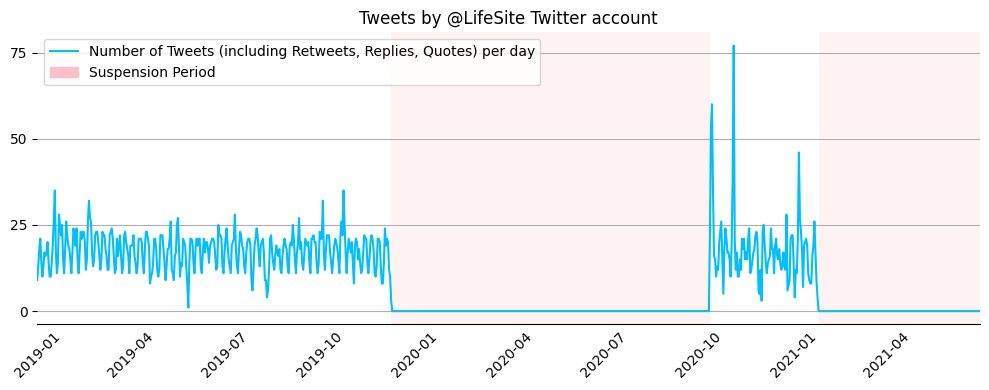
\includegraphics[scale=0.32]{../figure/lifesite_updated_legend.jpg} 
		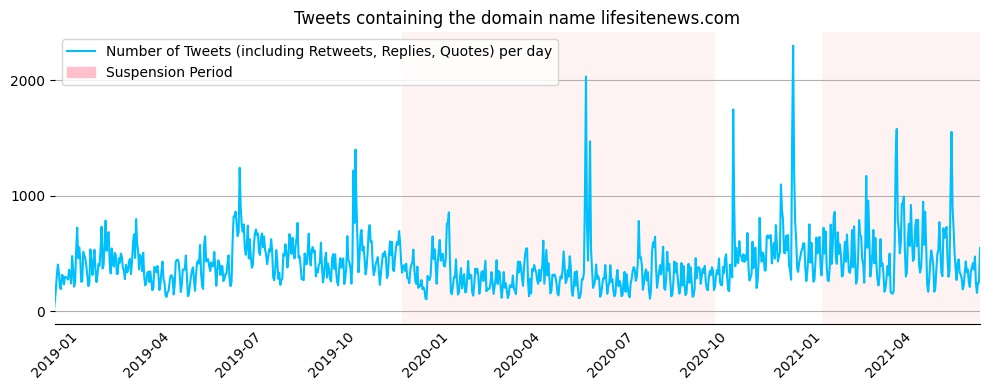
\includegraphics[scale=0.32]{../figure/lifesite_domain_updated_legend.jpg}
\caption{Top panel: number of Tweets (including Retweets, Replies, Quotes) per day of the Twitter account $@Lifesite$ linked to the website lifesitenews.com from January, 2019 until April 2021. Bottom panel: number of Tweets (including Retweets, Replies, Quotes) per day that have shared a lifesitenews.com URL link from January, 2019 until April 2021. }
\label{fig2}
\end{figure}

To assess the impact of this double temporary suspension, we also collected all the Tweets posted by other accounts, during the same period, including a url link with the domain name lifesitenews.com. 
The bottom panel of Figure \ref{fig2}, shows that during both periods of temporary suspension, other users still shared lifesitenews.com links and that the level was only slightly below the tweeting and retweeting levels prior to the first temporary suspension.
Suspending a Twitter account is an intervention which aims at penalising users, in order to make them respect the Twitter rules.  The activity of accounts linked to websites usually consists in sharing on social media their own published articles. 
The bottom panel of Figure \ref{fig2} points towards the limitations of suspending the Twitter account $@LifeSite$, because the 
articles published on lifesitenews.com were still being actively shared by other Twitter users. 
Finally, \cite{LifeSiteNews} has announced on their website that they were using alternative platforms in response to multiple suspensions on large platforms. 
Figure \ref{telegram} shows the creation of their Telegram channel in early 2021 and their level of activity throughout the second suspension period on Twitter, illustrating a case study of platform migration. 
It should be noted that the Number of followers on Telegram is 13.4k (Feb 2023) against 58.6k (Feb 2023) on Twitter. 
Finally, the Twitter account of LifeSiteNews has been recently activated in October 2022. 
\begin{figure}[h]
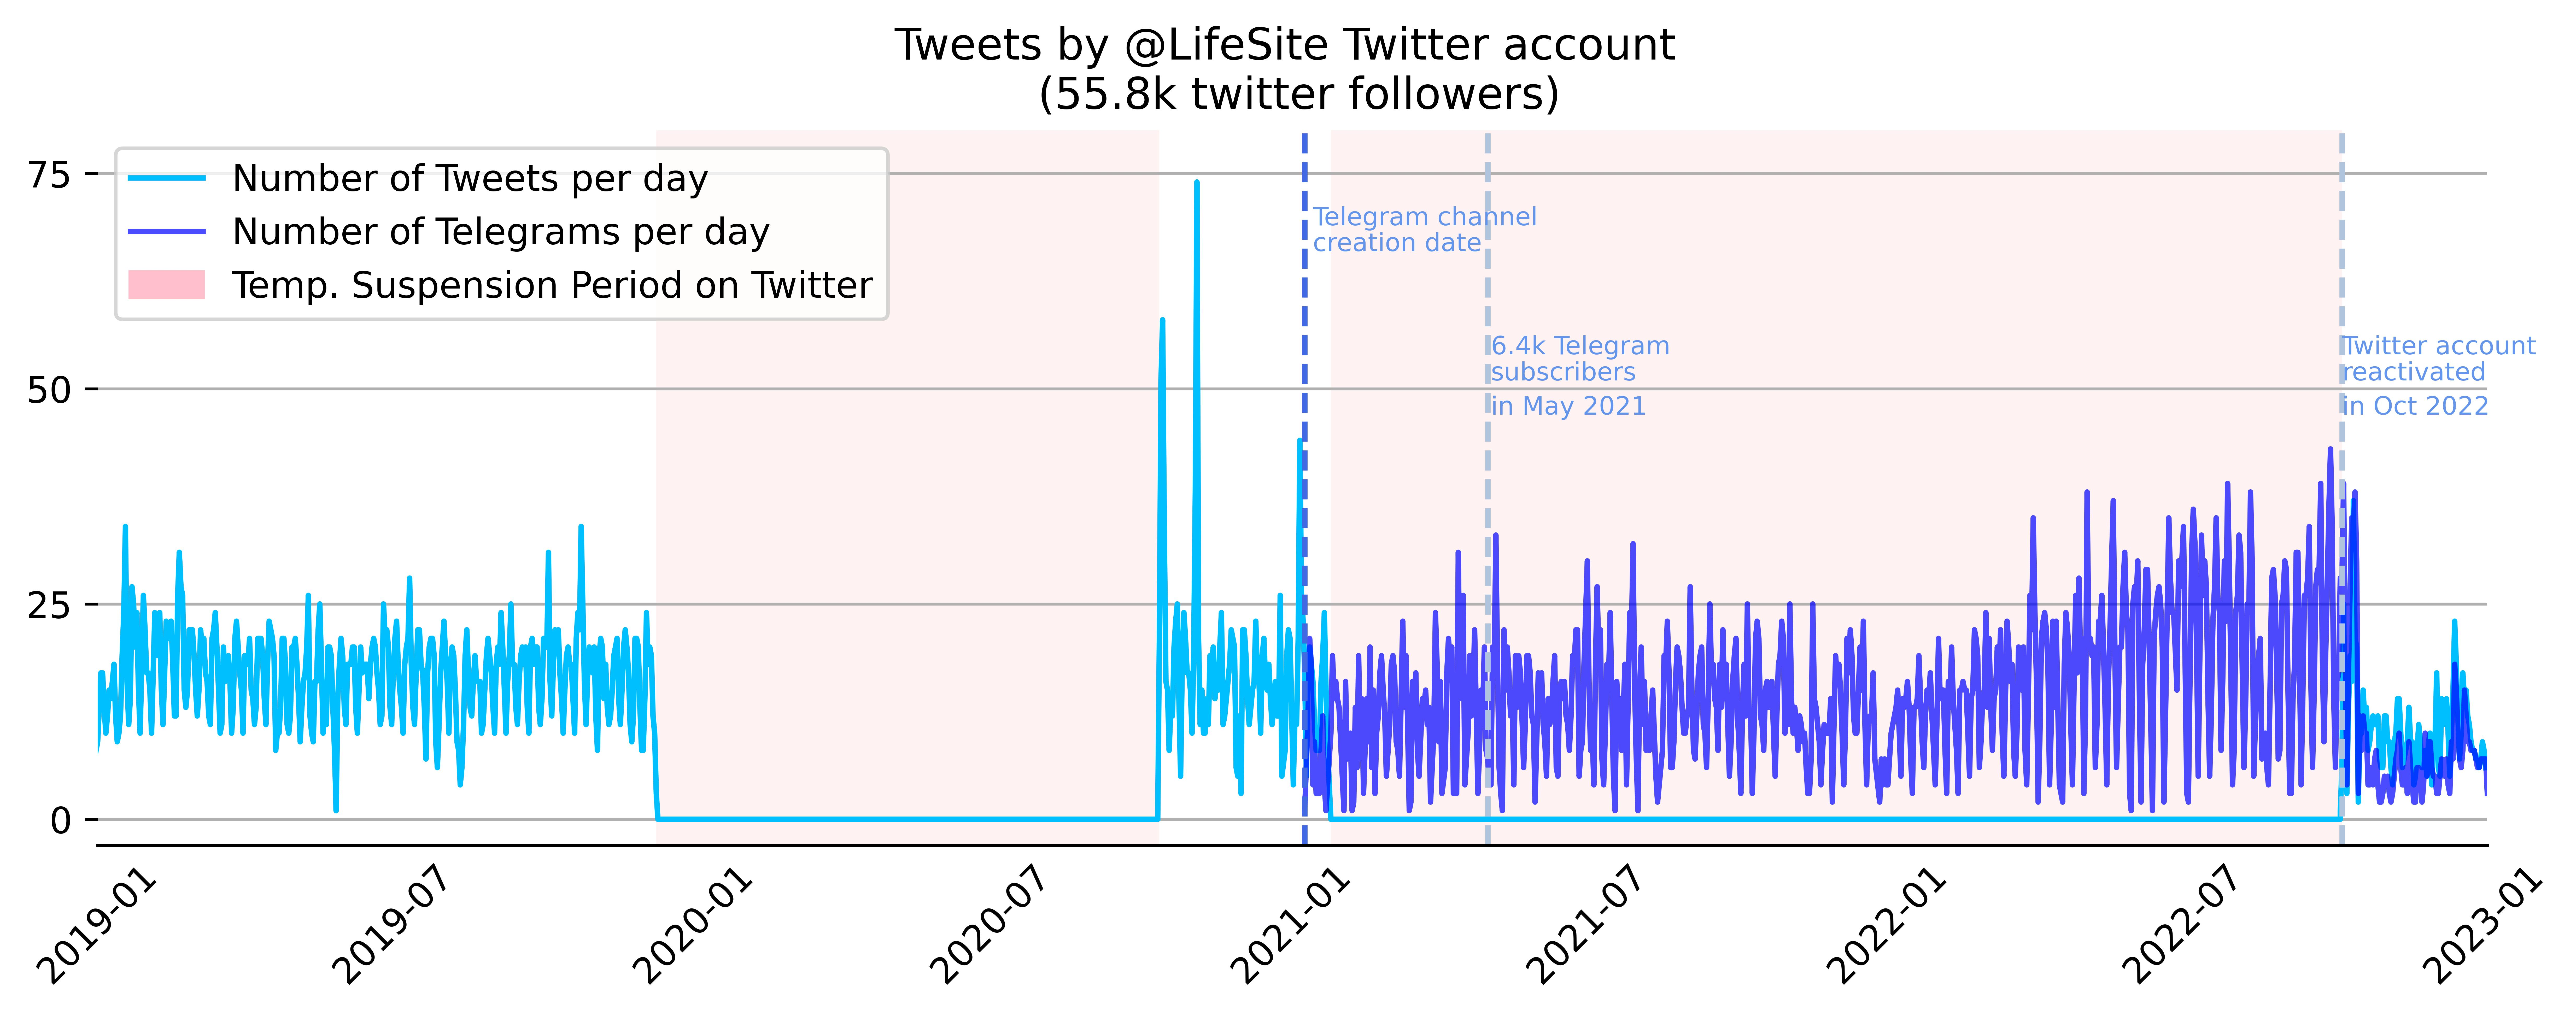
\includegraphics[scale=0.34]{../figure/lifesite_2022_01_04.jpg} 
\caption{Number of posts per day on the Telegram Public channel LifeSiteNews, created on January 9, 2021. }
\label{telegram}
\end{figure}

\subsection{YouTube}

Turning to YouTube, we investigate the case of the YouTube channel associated to  One America News Network, a cable news channel, with several failed fact-checks according to \cite{MBFCoann} and \cite{openfeedbackoann}. 
Their temporary suspension on YouTube in relation to medical misinformation was announced in several media outlets, see for example ~\cite{nbcnews}. 
We collected for this channel, the video count (number of uploaded videos) and the view count using the YouTube API v3, between November $2020$ and January $2021$.\endnote{For the video count, we used the {\it playlists} endpoint to retrieve the videos uploaded with their publishing date and for the view count we used the IDs of the videos we had from the playlists, then via the {\it videos} endpoint we retrieved the view count during the month of June $2021$.}

\begin{figure}[h]
\hspace{-2em}
		\includegraphics[scale=0.32]{../figure/delete_youtube_1_oann.png} \hspace{4em}
		\includegraphics[scale=0.33]{../figure/delete_youtube_2_oann.png} 
	\caption{Top panel: Number of YouTube videos uploaded each day by the youtube channel {\it One America news Network} November 1, 2020 and January 1, 2021. Bottom panel: accumulated view counts for videos. The metrics correspond to the videos’  publishing date and the data is retrieved from the YouTube API with the {\it playlists} and  {\it videos} endpoints. }
	\label{delete_youtube_oann}
\end{figure}

\smallskip

Figure \ref{delete_youtube_oann} shows the daily number of videos uploaded and their view count. 
We can clearly see the suspension period in the data, as the number of published videos is down to zero for one week after the strike announced by media outlets on November $24$, $2020$. 
When comparing the average view count during one week before the suspension and one week after the suspension, we observe a clear drop, while the video uploads one week and one week after where of the same magnitude.
%When comparing one month before and after the suspension, the view count decreased by -73\%. 
It is unclear wether this drop in view count is linked to a lower organic engagement or an algorithmic intervention by YouTube.
However, the activity of the channel in terms of videos uploads has drastically decreased by mid-December 2020 and was close to zero after March 2021. OANN's Twitter account has announced their migration from YouTube to Rumble on March 17, 2021 (see Figure \ref{tweets_about_yt_suspensions}). 
This case study illustrates on the short run some potential indirect effects of content moderation policies in terms of platform migration. 

\begin{figure}[h]
	\centering
		\includegraphics[scale=0.3]{./img/oann/fig3_oann.png}
		\caption{Tweet announcing OANN's migration to Rumble, Twitter ID \href{https://twitter.com/OANN/status/1372238828425998336}{1372238828425998336}.} 
	\label{tweets_about_yt_suspensions}
\end{figure}

\section{How can we investigate Flags, Notices and information panels?} \label{flags}

Platforms can provide more context to users by attributing a label or an information panel to a piece of content. This intervention is well documented in the literature, in terms of functioning, effectiveness and perception, see \cite{crawford2016flag}, \cite{morrow}, \cite{yaqub2020effects}, \cite{sharevski2021misinformation}, \cite{pennycook2020implied}. 
However information and data about whether a piece of content was flagged, labelled or contains an information panel is not available on official APIs. 
Hence it's challenging to understand the specific rules applied, whether content is labelled due to an algorithmic decision or users reports or moderators. 
In this section, for each platform, we rely on a set of links fact-checked as false and investigate whether they contained a flag, a label or an information panel. 
Since the information cannot be found on APIs the only way to investigate the presence of labels is by scraping publicly available content. 

\subsection{Facebook}

\begin{figure}[h]
\centering
\includegraphics[scale=0.35]{./img/fb_flags/fb_flag_1.png}
\includegraphics[scale=0.35]{./img/fb_flags/fb_flag_2.png}
\includegraphics[scale=0.49]{./img/fb_flags/fb_flag_3.png}
\caption{Examples of Facebook posts having shared a link fact-checked as False by one of Facebook’s partners. Screenshots taken on July 8, 2021.} 
\label{fb_flags}
\end{figure}
%\caption{Examples of Facebook posts having shared a link fact-checked as False by one of Facebook’s partners. Screenshots taken on July 8, 2021: \href{https://www.facebook.com/groups/1220117708132394/permalink/2386760061468147}{facebook.com/groups/1220117708132394/permalink/2386760061468147},  \href{https://www.facebook.com/groups/473809623000471/permalink/1333200093728082}{facebook.com/groups/473809623000471/permalink/1333200093728082}, \href{https://www.facebook.com/691911990845585/posts/3835629366473816}{facebook.com/691911990845585/posts/} \href{https://www.facebook.com/691911990845585/posts/3835629366473816}{3835629366473816} .} 
%No information or available fields regarding the Facebook flags can be found on Buzzsumo or CrowdTangle, the two APIs we use to access Facebook data. The only way to verify Facebook’s flagging policy is thus via scraping publicly available content. 

We first searched for all the Facebook posts having shared one specific link\endnote{ Click \href{https://beforeitsnews.com/eu/2021/04/stay-away-from-the-vaxxed-it-is-official-from-pfizers-own-documents-2671454.html}{here} to access the link and  \href{https://healthfeedback.org/claimreview/insufficient-evidence-to-claim-covid-19-vaccines-cause-menstrual-irregularities-in-vaccinated-women-vaccinated-people-arent-making-unvaccinated-people-ill/}{its fact-check by Health Feedback}.} rated as ‘False’ by Science Feedback, one of Facebook's fact-checking partners. We used the `search' endpoint available on the CrowdTangle API to search for these posts.
Doing so, we collected 20 Facebook posts. 
Then we scripted an adapted scraping code to verify whether they contained an information panel, a fact-check flag, both or none (see Figure \ref{fb_flags}). 
Three posts were unavailable, and thus could not be categorised by the scraper. %As Science Feedback has informed Facebook that they have assigned the rating ``False'' for this link, we expected that all these posts would contain a fact-check flag, but we had no expectations for the information banner. 

\begin{figure}[h]
\centering
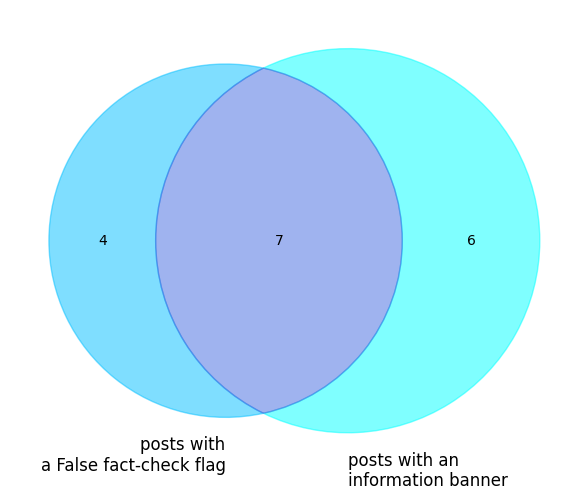
\includegraphics[scale=0.4]{../figure/facebook_pie_flags_updated.png}
\caption{Count of different flags for 17 Facebook posts who have shared the exact same link, fact-checked False by one of Facebook’s partners. }
\label{tab_flags_fb}
\end{figure}

Only $11$ posts out of the remaining $17$ had a ``False information'' flag, see Figure \ref{tab_flags_fb}. 
We observed that the flagged posts were also the ones in which the false link was expanded, which means that a banner was visible with an image of the linked article on which users can click. 
As the ‘False information’ flag is applied on the link banner, and not on the link itself when it appears in the text of a post, we found cases where a user is thus able to share a link fact-checked as ``False''  by one of Facebook's partners, without receiving a ``False'' flag if the link is not expanded, see Figure \ref{fb_flags}.
We could not identify why information panels ``Visit the COVID-19 Information Centre for vaccine resources", were applied on some posts and not on others, as we observed no clear difference in the content of the post in terms of keywords. 
It should be noted that some posts displayed both the information and the fact-check banners, as in the second panel of Figure \ref{fb_flags}.

\subsection{Twitter} 

When using the Twitter API V2, there is no field which indicates whether a Tweet contains a notice or not; with the exception of the interstitial ``possibly sensitive'' (see the top panel of Figure \ref{fig_notice}) and ``withheld" are both Tweet fields that can be recovered from the Twitter API V2. 
We take a deeper look at how notices and interstitials are introduced by Twitter. 
%links: $3$ $094$
%tweets $323$ $938$ 

First, we gathered a set of around $3$K  links redirecting to articles which were marked as ``False'' between April $2019$ and February $2021$ by Science Feedback. As a second step, we collected on June $30$, $2021$ all the Tweets that have shared at least one of these links, using minet~\cite{minet}. 
This tool was recently enriched upon our request via Github in order to capture whether a Tweet contains a notice or not, when using the ``minet twitter scrape'' command. 
The Tweet collection resulted in around $320$K Tweets, excluding Retweets. Only $28$ Tweets contained the notice { \it ``Get the facts about COVID-19''}, five Tweets contained the notice {\it ``Learn about US 2020 election security efforts''} and only one had the following notice {\it ``This claim about election fraud is disputed''}. 

Furthermore, we noticed that the labelling rule is not applied uniformly on a given set of Tweets sharing the exact same link. To illustrate, $657$ Tweets contained the exact same link redirecting to a video on Bitchute, entitled {\it Important information on coronavirus 5G Kung Flu}. 
Among those $657$ Tweets only three had the notice {\it ``Get the facts about COVID-19''} (see the bottom panel of Figure \ref{fig8}).
It might be that these three Tweets were the only ones reported by other users, since the labelling seems not to be automated with respect to a specific link redirecting to a fact-checked article. 
\begin{figure}[h]
\centering
		\includegraphics[scale=0.35]{./img/tweets/Capture_2021-06-30_2.png}
		\includegraphics[scale=0.32]{./img/tweets/Capture_2021-06-30.png}
	\caption{Two Tweets sharing the same link marked as ``False'' by Science Feedback, screenshots taken on June $20$, 2021. Top panel: a Tweet without an information notice. Bottom panel: a Tweet containing an information notice.}
	\label{fig8}
\end{figure}

\begin{figure}[h]
	\centering
		\includegraphics[scale=0.35]{./img/tweets/Capture_2021-07-01_2.png} 
		\includegraphics[scale=0.35]{./img/tweets/Capture_2021-07-01.png}
	\caption{Top panel: Tweet containing a URL link hidden behind an interstitial. Bottom panel: when clicking on $view$, to view the content hidden behind the interstitial in the top panel. Screenshots taken on July 1, 2021. }
	\label{fig_notice}
\end{figure}
%tweets possibly sensitive $9$ $344$
We further examine the placement of interstitials that indicate a possibly sensitive content. We find that around $9$K Tweets ($3\%$) out of the collected $320$K, contain the interstitial {\it ``potentially sensitive content''}. 
Again, to investigate whether the interstitial {\it ``potentially sensitive content''} is automated or not, we pick out one Tweet having shared a link\endnote{The link marked as False redirects to the article {\it 5G Technology and induction of coronavirus in skin cells – US National Library of Medicine (what David Icke has been saying for months) } and can be found \href{https://davidicke.com/2020/07/22/5g-technology-and-induction-of-coronavirus-in-skin-cells-us-national-library-of-medicine-what-david-icke-has-been-saying-for-months/}{here}.} marked as ``False'', which also contains the interstitial {\it potentially sensitive content} (see the top panel of Figure \ref{fig_notice}). 
There were $32$ Tweets that have shared the exact same link and only five of those Tweets contained the interstitial ``potentially sensitive content'', although they contained no graphic violence. To date, no data is available to verify whether some interstitials or notices were placed based on: Tweet reporting by other users or Twitter moderators or algorithmic rules or a mixture of all the previous.\endnote{Twitter Safety account announced in a Tweet (see Tweet ID : \href{https://twitter.com/TwitterSafety/status/1379515615954620418}{1379515615954620418}) on April 6, 2021 that their team ``will begin deploying automated tools to build on (their) efforts to label Tweets that may contain misleading information around COVID-19 vaccinations".}   
The appearance of interstitials may depend on the settings of a user's account and country or language specific regulations. In particular, in the settings of Twitter account, one can deactivate the display of interstitials for {\it sensitive content}, by ticking the box {\it Display media that may contain sensitive content} in the section {\it content you see}. 

\begin{figure}[h]
	\centering
	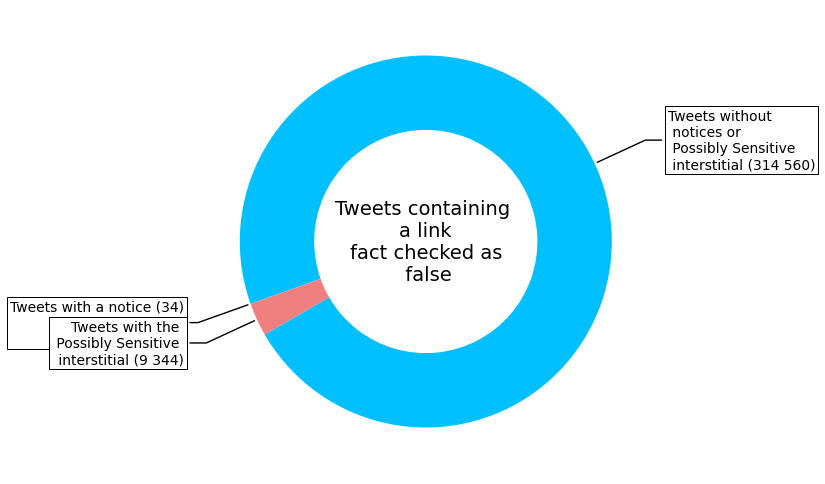
\includegraphics[scale=0.4]{../figure/donut_twitter_2022_01_04.png}
	\caption{Summary of the number of Tweets among the set of $323$ $938$ Tweets containing a link marked as False, by Science Feedback, which contain a notice or a Possibly sensitive interstitial or none.}
\label{flags_tab}
\end{figure}

\smallskip

Finally, the Tweets containing the interstitial ``potentially sensitive content'' widely outnumber the tweets which contain a notice (see Figure \ref{flags_tab}). 
We observed that among the Tweets which contain the interstitial {\it ``potentially sensitive content''}, there are Tweets which contain links redirecting to misleading articles about COVID-19 and yet they do not contain the label { \it ``Get the facts about COVID-19''}. 
The Twitter Help center explains the placement of interstitials of possibly sensitive content as follows: ``We may place some forms of sensitive media like adult content or graphic violence behind an interstitial advising viewers to be aware that they will see sensitive media if they click through''.  
However we noticed that the Tweets which contain the interstitial {\it ``potentially sensitive content''} do not necessarily contain graphic violent content, but rather links that redirect to articles marked as ``False'' by Science Feedback. 
It is possible that the possibly sensitive content interstitial is used as a type of soft moderation to reduce the visibility of a link. 

\subsection{YouTube} \label{youtube_panels}

To study the assignment of information panels to videos, we compiled a list of $170$ YouTube videos, fact-checked by Science Feedback between April $2019$ and March $2021$ and marked as containing inaccurate information. 
We collected the information panels, when present, under each video by scraping the content of the web page because this information is not available on the YouTube API. 
Several types of information panels were found, see Figure \ref{youtube_panel_screenshots}.

\begin{figure}[h]
	\centering
		\includegraphics[scale=0.1]{./img/youtube_panels/youtube_panel_covid.png} \vspace{0.3cm}
		
		\includegraphics[scale=0.1]{./img/youtube_panels/youtube_panel_covid_vaccine.png} 
		\vspace{0.3cm}
		
		\includegraphics[scale=0.1]{./img/youtube_panels/youtube_panel_climate.png}
	\caption{Examples of YouTube information panels displayed under Youtube videos respectively about: \href{https://www.youtube.com/watch?v=O1cFVdC2rZQ}{COVID-19}, \href{https://www.youtube.com/watch?v=v0-6JTr2Ifo}{COVID-19 Vaccine} and \href{https://www.youtube.com/watch?v=4U8kgiiVj5Q}{climate change}. The videos were accessed on September 2, 2021.}
	\label{youtube_panel_screenshots}
\end{figure}

\begin{figure}[h]
	\centering
		\includegraphics[scale=0.2]{../figure/youtube_pie_flags.png}
		\caption{Summary of the number of YouTube videos which contain an information panel, among the set of videos marked as false by Science Feedback.}
\label{youtube_panel_proportions}
\end{figure}

\begin{figure}[h]
	\centering
		\includegraphics[scale=0.22]{./img/youtube_panels/graph_no_banner.png}
		\vspace{0.4cm}
		\includegraphics[scale=0.22]{./img/youtube_panels/graph_with_banner.png} 
	\caption{Screenshots showing two duplicates of the same video, taken on July 21, 2021. 
Top panel: a \href{https://www.youtube.com/watch?v=d9GbVZOcT18}{YouTube video} about COVID-19 without an information panel. 	
Bottom panel: a \href{https://www.youtube.com/watch?v=A4RvrEKoNxc}{duplicate of the same video} uploaded under a different title and with a `COVID-19 vaccine' information panel.}
	\label{duplicates_yt}
\end{figure}

\smallskip

Almost half (46 \%) of the YouTube videos fact-checked as misleading by Science Feedback, were shown without any information panel (Figure \ref{youtube_panel_proportions}).
For the remaining videos, the most frequent information panel were COVID-19 (42 \%), followed by COVID-19 vaccine (9 \%), which is probably linked to a higher likelihood of fact-checking medical misinformation given the ongoing events at that time.
We noticed that the same video was sometimes uploaded multiple times with different YouTube links and different titles. 
One YouTube link might contain an information panel while its duplicates did not, see Figure \ref{duplicates_yt} for an example.  
In addition, we noticed that some keywords in the video titles were often associated with an information panel, such as ``COVID-19", ``coronavirus", ``pandemic" and ``testing", while some notational variants like ``C O V I D 19" or ``Cv19" were not associated with a panel.
Therefore, we suspect that YouTube is automatically adding information panels based on the presence of certain keywords in the video title and maybe in the video description, independently of the content of the video.
Note that in Figure \ref{duplicates_yt}, the video with ``C.O.V.I.D.19" in its title had an information panel, hinting that YouTube might adapt its list of keywords as new notational variants for COVID-19 appear or that some information panels might be added manually, by content content moderators or following users' reports or a mixture of the previous.


\section{Can we investigate algorithmic reduction of visibility of posts or accounts?}
We turn to the last family of content moderation policies linked to misinformation: reducing the visibility of a piece of misleading content as a mean of soft moderation. It is often referred to as ``shadow banning". Given the abundance of content, opting for this intervention allocates to algorithms the role of gatekeepers and it raises several concerns. This is because,  algorithmic interventions linked to misinformation are hard to investigate. On the one hand, by design these interventions are undetectable by the public eye and on the other hand the algorithmic rules used are not transparent. \cite{kokil2023silenced} investigate ``shadow banning" on Twitter and their findings show that it remains a rare event. \cite{LEERSSEN2023105790} discusses visibility reduction from a legal perspective and outlines the challenges related to accountability in relation to the Digital Services Act in the EU. In this section, again based on media outlets with failed fact-checks, we provide several illustrations and methodologies to investigate this intervention. 

\subsection{Facebook} \label{reduce_fb}

First, we investigate the famous case of the website $Infowars$. This website appears in the Misinformation Directory by \cite{misinformationdirectory}, it also has {\it very low}  factual reporting according to \cite{MBFCinfowars} and several failed fact-checks reported by \cite{openfeedbackinfowars}.  \cite{facebookinfowars} explicitly stated the following: {\it ``While much of the discussion around Infowars has been related to false news, which is a serious issue that we are working to address by demoting links marked wrong by fact checkers"}. According to a news article published on May 2, 2019 by \cite{wiredalexjones}, Facebook announced that they would prohibit users from sharing Infowars content unless, they are explicitly condemning the material.

To audit this intervention, we used the ``/posts/search'' endpoint of the CrowdTangle API and  collected $37~242$ Facebook public posts containing the domain name ``infowars.com'', published between January $1$, $2019$ and December $31$, $2020$. We found in the collected data some Facebook posts that did not directly share an Infowars link, but rather a YouTube or Facebook video containing an Infowars link in its description. Thus we excluded such posts from our data and kept $27$ $721$ posts directly sharing an Infowars link.

\begin{figure}[h]
\hspace{-2em}
		\includegraphics[scale=0.32]{../figure/facebook_crowdtangle_infowars_1.png}
		\includegraphics[scale=0.32]{../figure/facebook_crowdtangle_infowars_2.png} 
	\caption{Public Facebook posts sharing an Infowars link in $2019$ and $2020$ collected from the CrowdTangle API. The red line marks the date of May $2$, 2019, when Facebook has announced the ban regarding Infowars. top panel: Number of daily posts. Bottom panel: Engagement metrics: average number of reactions, shares and comments per post. }
	\label{infowars1}
\end{figure}

The number of public posts sharing an $Infowars$ link remained globally stable throughout $2019$ (see Figure \ref{infowars1} top panel). 
Thus the measure announced by Facebook does not seem to have prevented users from sharing an $Infowars$ link. Nevertheless, a clear drop in engagement was observed on May $2$, $2019$ (see Figure \ref{infowars1} bottom panel). 
The number of reactions, shares and comments per post have decreased respectively  by $-94\%$,  $-96\%$ and $-93\%$  when comparing the two months before and after May $2$, $2019$. This suggests the measure taken by Facebook in May $2019$, is not a ban per se, but rather a $reduce$ measure. This is because users could still post $Infowars$ links, but these posts generated less engagement. It should be noted that the engagement metrics increased again by the end of $2019$ / beginning of $2020$, suggesting that the $reduce$ measure may have been lifted a few months after its implementation.

\subsection{Twitter}  \label{globalresearch}

Turning to Twitter, we present a case study where two interventions that reduce the visibility were applied at the same time. We investigate the case of the website $globalresearch.ca$, with a low factual-reporting according to \cite{MBFCgloabalresearch} and which is linked to the Twitter account {$@CRG\_CRM$} (indicated on their website). 

When a user searches via the Twitter search-box for the domain name $globalresearch.ca$, no results appear as shown in the screenshot in the top left panel of Figure \ref{fig3}, taken on June $14$, $2021$. To investigate whether this was an intervention or simply no Tweets contained this domain name, we searched via the Twitter API v2 for Tweets with the query {\it globalresearch.ca} three months before and after the date of the screenshot. We found a strictly positive number of Tweets containing this domain name with strictly positive engagement metrics, as shown in the top and bottom panel in Figure \ref{fig4}. It's likely that users who post Tweets including articles from the {\it globalresearch.ca} website receive Tweet level engagement from their own followers. Furthermore when a user attempts to click on a link which contains {\it globalresearch.ca} in a Tweet (top right panel in Figure \ref{fig3}), a warning message appears and indicates that the link may be unsafe (bottom left panel \ref{fig3}) - hence acting as a second layer of visibility reduction. Furthermore, we noticed on May $25$, 2021 that the Twitter account {$@CRG\_CRM$} linked to the website $globalresearch.ca$ was suspended, see the bottom right panel in Figure \ref{fig3}. 

For the case of this Twitter account and the linked website, it is likely that a mix of interventions was used: reducing the visibility via the search box, reducing the visibility by introducing a warning message and suspending the related Twitter account.  

\begin{figure}[h]
\centering
	\includegraphics[width=3.7cm, height=2.5cm]{./img/globalresearch_14_06_2021_16pm_UTC.png}  
	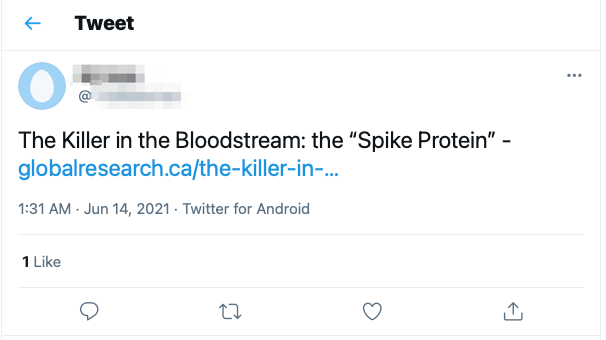
\includegraphics[width=3.7cm, height=2.5cm]{./img/globalresearch/tweet.png} 
	\includegraphics[width=3.7cm, height=2.5cm]{./img/globalresearch/warning.png} 	
	\includegraphics[width=3.7cm, height=2.5cm]{./img/globalresearch/globalresearch_2021-06-14.png}
	\caption{Screenshots taken on June 14, 2021. Top left panel: no results can be found when searching for Tweets with the domain name $globalresearch.ca$ via the Twitter search box. Top right panel: example of a Tweet containing the domain name {\it globalresearch.ca}. Bottom left panel: warning message that appears when a user attempts to click on a link which contains the domain name {\it globalresearch.ca}. Bottom right panel: account suspension message of $@CRG$\_$CRM$ linked to {\it globalresearch.ca}.}
		\label{fig3}
\end{figure}

\begin{figure}[h]
\centering
\hspace{-2em}
		\includegraphics[scale=0.4]{../figure/globalresearch_domain_2021-08-17.jpg}  		\includegraphics[scale=0.4]{../figure/globalresearch_domain_engagement_2021-08-17.jpg}
\caption{Top Panel: daily number of Tweets, excluding Retweets, containing the query {\it globalresearch.ca} from January $1$, $2021$ until June $30$, $2021$. Bottom Panel: engagement metrics of Tweets containing the query {\it globalresearch.ca} from January $1$, $2021$ until June $30$, $2021$. Data collected via the Twitter API v2 on August $17$, 2021.   }
\label{fig4}
\end{figure}

\subsection{YouTube}

YouTube can reduce the visibility of certain videos via its recommendation system, namely by recommending content from authoritative sources. They also state that they set out to prevent their systems from serving up content that could misinform users in a harmful way, particularly in domains such as science, medicine, news, or historical events.

To investigate how recommendations can be used to reduce the visibility of potentially harmful and misleading content, we designed an experiment that simulates a user's behaviour on YouTube using an automated program. The results are to be explored with caution as no clear instructions about how exactly the recommendation algorithms of YouTube address videos identified as misleading. 
\subsubsection{Experiment description.} 
We used a list of $45$ YouTube videos marked as {\it False} by Science Feedback and classified under the category ``health''.
First, we visit the YouTube videos marked as ``False'' from our list of videos and a clean watch history.
Second, for each YouTube video (parent), our automated program collects around $20$ recommendations\endnote{When we visit a video, we get a number of recommendations that vary between $18$ videos and $22$ videos.} and clicks on the top $10$ videos (children) in sequential order. 
Third, for every video in the set of the top $10$ recommended YouTube videos (children), we collect their own top $20$ recommended videos (grand-children).
In addition, to simulate a user's behaviour, the automated program watches each video for a few minutes. If the video duration is ten minutes or less, the automated program watches the whole video. If the video duration is strictly higher than ten minutes, then the automated program watches only five minutes.
\subsubsection{Experiment results.} 
Doing so, we collected $10~549$ recommended YouTube video entries, among which $3~895$ were unique. 
To analyse the collected data, we look for videos belonging to medical misinformation: $(i)$ at the channel level and $(ii)$ at the video level. 

The $3~895$ unique YouTube videos belonged to $1~562$ unique channels, and then we counted the number of times videos from each channel got recommended.
Figure \ref{reduce_youtube} shows the top ten recommended channels, whose videos represent $30\%$ of the recommendations.
Fox News and Sky News Australia - which both have a ``mixed'' factual reporting level according to the website \cite{MBFCfoxnews} with several failed fact-checks - are at the first and third place respectively.
PragerU - a website with a ``low" level of factual reporting according to \cite{MBFCprageru} - is also among the list of the ten most recommended channels. 

\begin{figure}[h]
	\begin{center}
		\includegraphics[scale=0.45]{../figure/reduce_youtube.png} 
	\end{center}
	\caption{Top ten channels recommended by YouTube when we simulated a user that starts by watching a video fact-checked as False and then follows the top recommendations.}
	\label{reduce_youtube}
\end{figure}

Furthermore, we ranked the videos based on the number of times they got recommended and asked Science Feedback to fact-check the top 40 recommended videos. 
Those videos were recommended $1~735$ times, which represents $16\%$ of the total recommended videos.
Among the 40 examined videos, four videos were marked as {\it misleading} and they were recommended $132$ times out of the $1~735$ recommendations (i.e. $7.7\%$).
Four other videos were marked as {\it hyper-partisan} and they were recommended $184$ times (i.e. $10.7\%$).
As we collected the recommendations of misinformation videos, we expected to find a high proportion of videos of questionable content.
But only {$18.4\%$} of the recommendations corresponded to $misleading$ or {\it hyper-partisan} videos.
This relatively small percentage hints towards that idea that YouTube is probably reducing the visibility of videos containing misinformation. 
However, when we investigated misinformation at the channel level, we found that videos belonging to channels that are not highly authoritative were being recommended.
It might be that the recommendation system of YouTube is reducing the visibility at the video level but not necessarily at the channel level. These findings are preliminary and experiments on larger sets of potentially misleading YouTube videos need to be conducted. 

\section{Discussion}

In this article we have assessed three broad categories of interventions to tackle misinformation by Facebook, Twitter and YouTube: $(i)$ suspension of accounts, $(ii)$ introduction of flags, labels and information panels and $(iii)$ reducing the visibility of content. Mainstream platforms such as Facebook, Twitter and Youtube are increasingly working towards higher data transparency. 
Yet the present research sheds light on the restrictions to access data and its limits, which impede the academic community from studying successfully online misinformation and assessing the impact and pertinence of platforms' interventions regarding this phenomenon. 
In this section, we provide a discussion regarding the limitations to access data and the lack of transparency regarding misinformation related interventions. 

\subsection{A need for complete \& pertinent data}

When Facebook, Twitter or YouTube intervene by suspending an account, the data can no longer be accessed via scraping or via official APIs (Twitter, YouTube, CrowdTangle) for the purposes of scientific research. This hampers the investigation of how platforms moderate content, especially content deletion which is often perceived by users as censorship.

For example, the original list of YouTube videos with failed fact-checks (summarized in Figure \ref{youtube_panel_proportions}), had over $200$ YouTube videos available in March $2021$. 
However, by June $2021$, thirty videos had disappeared from the YouTube API for policy violation and we could no longer examine them. 
To avoid interrupting research following data deletion by a given large platform, it seems essential to make available at least some metadata of the content posted by the suspended accounts.

Currently it is impossible to study permanent deletions using available social media data but they could be investigated indirectly (and imperfectly) using an adapted methodology.
Following the Capitol riots in January $2021$, \cite{twitterdc} has announced the suspension of more than $70~000$ accounts related to QAnon.
A BBC journalist has recently shared in a \cite{tweetBBC}, the effects of this measure by counting the number of times hashtags related to the QAnon movement have been used over time, such as \#QAnon or \#WWG1WGA.
A drastic reduction in hashtag use was found when comparing the first quarter of $2021$ with the first quarter of $2020$.

However, data can also disappear due to other factors independent of platforms' content moderation policies and it is hard to identify how much of the drop in QAnon related hashtags is due to the Twitter intervention or to accounts migrating to other platforms or simply a drop in using the hashtag for other unidentified factors.
To illustrate, \cite{mcminn2013building} collected $120$ million Tweets related to general topics. 
The same published set of Tweet IDs was then used by \cite{mazoyer2020french}. The authors ran the same Tweet collection in $2018$ and they only found $67$ millions of Tweets (55\%). The authors argue that this drop is probably due to Tweets having been removed by users and Twitter accounts being shut by the users themselves.
As data can disappear from platforms over time, it is hard to distinguish whether platforms or users are the ones responsible for data removal. Hence it is essential that platforms communicate this information via Tweet metadata so that the academic community can assess rigourously content deletion related to content moderation.

Aside from the disappearance of data due to content moderation, some essential metrics for the study of misinformation are not accessible via main APIs. 
In particular, the $reach$ of posts on Facebook, which is the number of people who actually see a given post, cannot be recovered from the CrowdTangle API. Hence, researchers can only build proxies for this metric based on available data, such as engagement metrics. The reach, impressions or view count is an essential metric to assess ``viral" content, as the number of users who see a post is generally different from the number of users who engage with a post.  Notice that this metric was recently made available via the Twitter API since December 22, 2022. 

Furthermore, to the best of our knowledge, fields related to flags, notices and information panels are not available on the official APIs, with the exception of the {\it withheld}  and {\it possibly sensitive content} interstitials in the Twitter API v2. This information does not seem to be sensitive and can be very useful for misinformation research studies to asses the impact and pertinence of information panels on a larger scale. To illustrate, information panels on YouTube, Twitter and Facebook have been used in the US for elections integrity following the controversy about elections' results. \cite{therodefacto} shows in a research note that information panels have been placed under YouTube videos including political figures, during the 2022 French presidential elections, while there was no controversy regarding the results. More research needs to be conducted to assess the pertinence of US-centric interventions when the targeted users are in other geographic zones.  

Finally, there are growing restrictions to access APIs, see \cite{api}.
In April $2018$, likely as a response to the Cambridge Analytica scandal, \cite{facebookdata} severely limited the access to their official APIs, see the commentary by \cite{bernhard}.  
CrowdTangle is today a reliable source for researchers, journalists and the civil society to access Facebook data. 
To illustrate, CrowdTangle has been recently used by \cite{theeconomist} to show that Facebook might be disproportionally favouring highly partisan information. Along the same lines, the Twitter account \cite{facebookstop10} shows each day the ten top performing link posts by U.S. Facebook pages in the last 24 hours, where right leaning sources such as Fox news or Breitbart appear often. 
\cite{facebookapptop10} has reacted to such rankings based on CrowdTangle data, by saying that {\it ``Ranking top Page posts by reactions, comments, etc. doesn’t paint a full picture of what people actually see on Facebook"}. There is a general suspicion that access to Facebook data might be further restricted in a near future, see for example the articles by \cite{nytimestheshift} in the New York Times or \cite{bloomberg} in Bloomberg. Regarding the other large platforms, \cite{twitterdev} has recently announced restrictions to access their API by no longer supporting free access, even for their academic track.  

\subsection{A need for meaningful transparency.} 
Large platforms populate their own transparency centres and provide aggregate figures by policy area. When navigating through the categories of policy areas in available enforcement reports, by Facebook, YouTube or Twitter, to the best of our knowledge, misinformation is absent from the data available on their transparency centres - in spite of clear evidence that content that is considered as misleading and harmful is actioned by these platforms.  
Platforms' official communication about misinformation interventions is scarce and researchers, journalists and the civil society, usually discover interventions related to misinformation via monitoring social media accounts related to domain names with several failed fact-checks or via articles in news outlets. 

We are aware that full transparency regarding operational aspects of misinformation related interventions can backfire.
This is because the aimed users might find ways to circumvent the interventions, for example by using notational variants that algorithms might use to target content. 
But, a balance needs to be found so that stakeholders can understand how the platforms are regulating content. 

In certain cases, the platform interventions were not motivated by content moderation to limit misinformation, but rather by other rule violations. To illustrate, when \cite{facebookinfowars} removed four pages related to the InfoWars website, the cited reason was repeated violations of Community Standards: 
{\it ``While much of the discussion around Infowars has been related to false news, which is a serious issue that we are working to address [...], none of the violations that spurred today’s removals were related to this''}.

In the previous example, the compagnies' communication was very clear about the reason of the interventions. 
However, very often no official communication on behalf of the platforms can be found for specific interventions observed in collected data. 
Because misinformation is often associated with creating fake accounts to speed its spread, and incitation to violence, it is sometimes unclear to distinguish between interventions due to misinformation and interventions due to other guideline violations, and more transparent communication on platforms' actions would help monitor the interventions specifically related to misinformation. Platforms could explicitly provide via metadata the specific policy violation rather than just displaying on a piece of deleted content that the rules were violated.

\subsection{A need for independent audits} 
%dynamic aspect : changing rules covid. changing algorithms. 
%rules clear? 
%centralised internet 
To date, research about content moderation policies of very large online platforms related to misinformation is still scarce, mainly due to data and information availability as we have shown in the present research paper. 

Large platforms choose today in a central and rather opaque matter which rules to set, facing pressure from the market due to multiple accusations of not providing a safe and healthy online space. These policies are de facto ``terms of service" of a small number of private companies that dominate the market,  that users are bound to respect.
But they raise the question of the choice of a model of governance to be adopted within these online spaces because they are frequented daily by millions (sometimes billions) of users around the world, with different values and perceptions of freedom of expression. 
The current model of self-regulation, where platforms create the rules, implement them and audit them themselves by publishing aggregate figures via their transparency centres is no longer satisfactory to many stakeholders. 
Especially that the rules evolve often as a function of ongoing events, such as the recent COVID-19 pandemic.
 
In a sense, reflecting on large platforms governance is both a contradiction and an aporia. On one hand, it can come as a contradiction,  because in the spirit of the internet pioneers, the members of the online community had their own values and their own way to self regulate (see for example \cite{barlow}) and the {\it code} or architecture was itself a sufficient mean to protect newly acquired freedoms, \cite{lessigcode1}. On the other hand, it is an aporia, because online spaces have drastically changed  and the high concentration of usage within few very large platforms gave rise to many new unforeseeable challenges, such as harassment, hate speech and harmful misleading content. Since these challenges concern millions of users around the world, it seems necessary that third parties take part in assessing and evaluating the pertinence and effects of content moderation policies. The methods presented in this paper can help to monitor not only the platforms' actions against misinformation, but also their subsequent consequences in real-life settings.

%It is also possible that platforms usually follow specific rules on how to fight misinformation, but that sometimes the sudden media coverage of specific events leads them to take exceptional actions, such as with the Capitol riots and Trump's suspension from Facebook, Twitter and YouTube.
%We would argue that policies should be clearly stated and carefully designed, rather than implementing interventions on a case-by-case basis and in response to the latest news events.

%It was shown that credibility indicators do reduce misperceptions and sharing, although their impact varied vastly depending on the presentation of the warnings, see \cite{yaqub2020effects} and \cite{sharevski2021misinformation}.
%Moreover \cite{pennycook2020implied} show that such sparse application of warnings can lead to an ``implied truth'' effect, where users may assume that content without warnings have actually been verified and shown to be true.
%Using a different approach, \cite{mosleh2021perverse} identified Twitter users sharing false news and replied to their false Tweets with links redirecting to fact-checking websites.
%They observed a decrease in the quality and accuracy of the content subsequently shared by the corrected user. 
%These research papers highlight the necessity to investigate the effects of content moderation policies linked to misinformation. 


%{\color{red} \bf Ouverture TikTok, }

\theendnotes

\bibliography{proj1}{}
\bibliographystyle{SageH}



\section{Appendix}

\noindent {\bf Acknowledgments} \\
We thank our colleagues at Sciences Po m\'{e}dialab for their feedback and suggestions, especially Dominique Cardon, Manon Berriche and Valentine Crosset. \bigskip

\noindent {\bf Funding} \\
This research was supported by the Make Our Planet Great Again’ French state aid managed by the Agence Nationale de la Recherche under the ’Investissements d’avenir’ program with the reference ANR-19-MPGA-0005. \bigskip

\noindent {\bf Competing interests } \\
We have no conflicts of interest to disclose. \bigskip

\noindent {\bf Ethics} \\
The data collection and processing complied with the EU General Data Protection Regulation (GDPR).\bigskip

\noindent{\bf Data availability} \\
The code needed to collect the data and create the figures is available on the following public GitHub repository: \href{github.com/medialab/webclim misinformation_related_interventions}{github.com/medialab/webclim\_misinformation\_related interventions}.

\end{document}
